% ================================= chapter 5 ================================= %
\chapter{実験}

\subsection{実験装置}
本実験で用いる実験装置を図??に示す。この実験装置は第\ref{chapter_modeling}章で示した実験装置と
同様の機能を有する。

\begin{figure}[htbp]
    \begin{center}
        %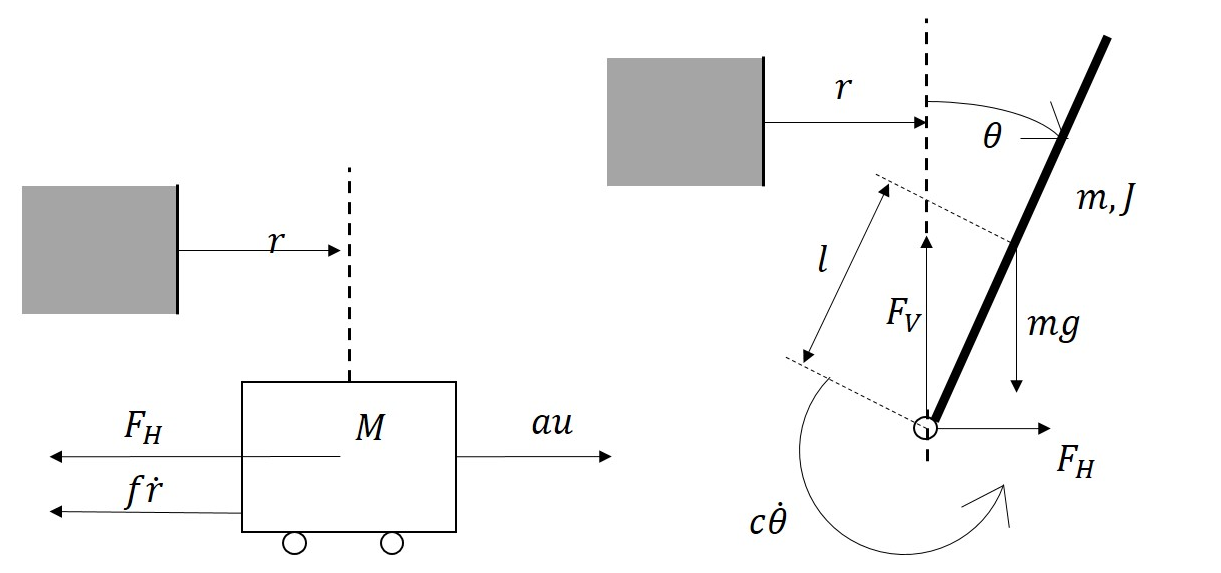
\includegraphics[width=0.6\linewidth]{modeling.eps}
        %\caption{図\ref{modeling}: モデリングのための力の分解}
        %\label{modeling}
    \end{center}
\end{figure}


\subsection{安定化制御の実験}
表??から表??までのパラメータを用いて、目標値変更における安定化制御を行う。
振子が鉛直上向きの状態から安定化制御を開始し、$5$秒ごとに台車の目標値を
$0.0 \to 0.5 \to 0.0$[m]と交互に切り替える。



\subsection{重み行列}

\subsection{オブザーバの極}

\subsection{サンプリング周期}

\subsection{シミュレーションと実験結果の比較}
表\ref{sim_exp}をもとに、シミュレーションと実験結果を比較した図を、図??から図??に示す。

\begin{table}[htbp]
	\begin{center}
    \caption{表\ref{sim_exp}: シミュレーションと実験の比較に用いるパラメータ}
		\begin{tabular}{|c|c|c|c|} \hline
			パターン & 重み行列$Q$ & オブザーバの極$P$ & サンプリング周期$dt$ \\ \hline\hline
			パターン01 & diag(1.0E6, 1.0E5, 1, 1) & (-23, -23) & 0.01  \\ \hline
			パターン02 & diag(1.0E6, 1.0E5, 1, 1) & (-50, -50) & 0.01  \\ \hline
			パターン03 & diag(1.0E6, 1.0E5, 1, 1) & (-23, -23) & 0.005 \\ \hline
			パターン04 & diag(1.0E6, 1.0E5, 1, 1) & (-50, -50) & 0.005 \\ \hline
			パターン05 & diag(1.0E5, 1.0E6, 1, 1) & (-23, -23) & 0.005 \\ \hline
			パターン06 & diag(1.0E5, 1.0E6, 1, 1) & (-50, -50) & 0.005 \\ \hline
			パターン07 & diag(1.0E5, 1.0E6, 1, 1) & (-23, -23) & 0.01  \\ \hline
			パターン08 & diag(1.0E5, 1.0E6, 1, 1) & (-50, -50) & 0.01  \\ \hline
			パターン09 & diag(1.0E6, 1.0E6, 1, 1) & (-23, -23) & 0.01  \\ \hline
			パターン10 & diag(1.0E6, 1.0E6, 1, 1) & (-50, -50) & 0.01  \\ \hline
			パターン11 & diag(1.0E6, 1.0E6, 1, 1) & (-23, -23) & 0.005 \\ \hline
			パターン12 & diag(1.0E6, 1.0E6, 1, 1) & (-50, -50) & 0.005 \\ \hline
		\end{tabular}
		\label{sim_exp}
	\end{center}
\end{table}

% --- patter 01 --- %
\begin{figure}[htbp]
    \begin{minipage}{0.5\hsize}
        \begin{center}
            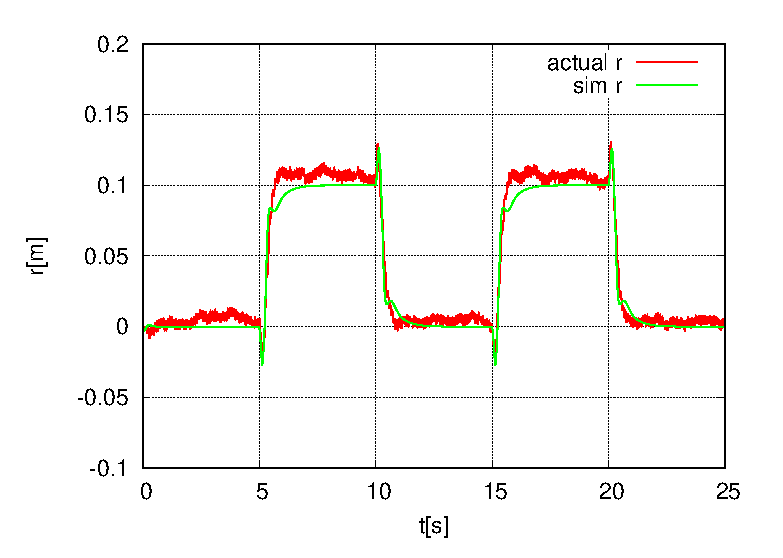
\includegraphics[width=1.0\linewidth]{case1_r.eps}
            \caption{図\ref{case01_r}: パターン01の台車位置}
            \label{case01_r}
        \end{center}
    \end{minipage}
    \begin{minipage}{0.5\hsize}
        \begin{center}
            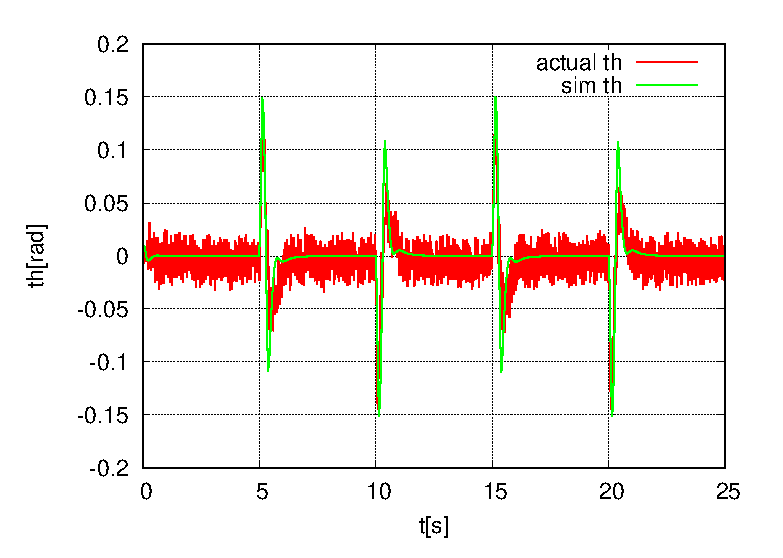
\includegraphics[width=1.0\linewidth]{case1_th.eps}
            \caption{図\ref{case01_th}: パターン01の振子角度}
            \label{case01_th}
        \end{center}
    \end{minipage}
\end{figure}

% --- patter 02 --- %
\begin{figure}[htbp]
    \begin{minipage}{0.5\hsize}
        \begin{center}
            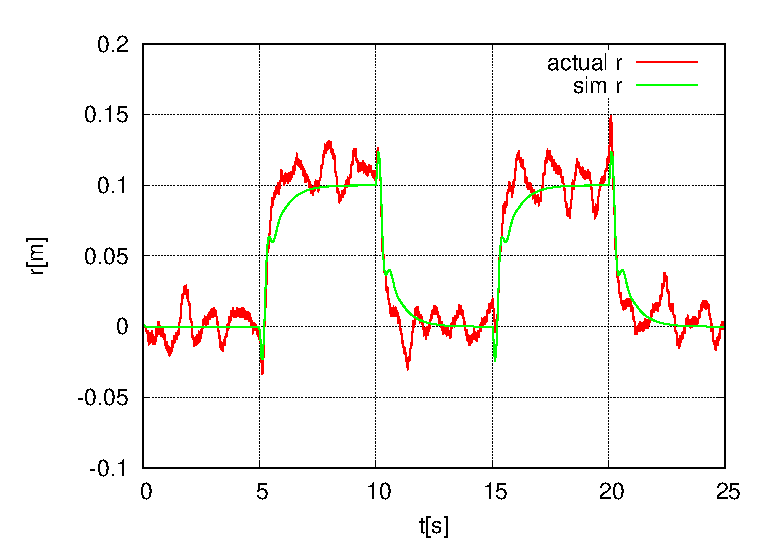
\includegraphics[width=1.0\linewidth]{case2_r.eps}
            \caption{図\ref{case02_r}: パターン02の台車位置}
            \label{case02_r}
        \end{center}
    \end{minipage}
    \begin{minipage}{0.5\hsize}
        \begin{center}
            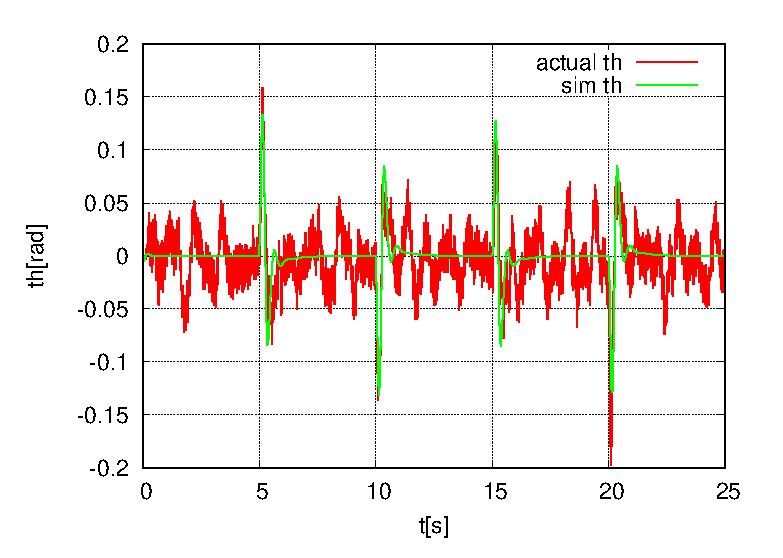
\includegraphics[width=1.0\linewidth]{case2_th.eps}
            \caption{図\ref{case02_th}: パターン02の振子角度}
            \label{case02_th}
        \end{center}
    \end{minipage}
\end{figure}

% --- patter 03 --- %
\begin{figure}[htbp]
    \begin{minipage}{0.5\hsize}
        \begin{center}
            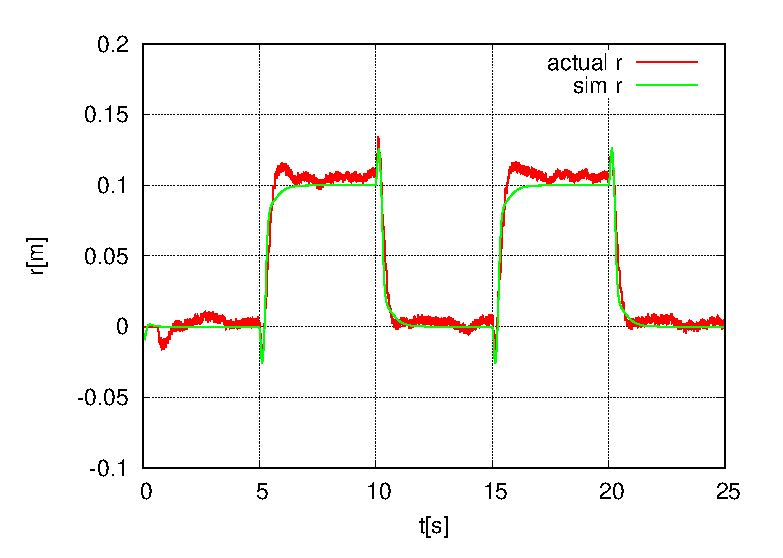
\includegraphics[width=1.0\linewidth]{case3_r.eps}
            \caption{図\ref{case03_r}: パターン03の台車位置}
            \label{case03_r}
        \end{center}
    \end{minipage}
    \begin{minipage}{0.5\hsize}
        \begin{center}
            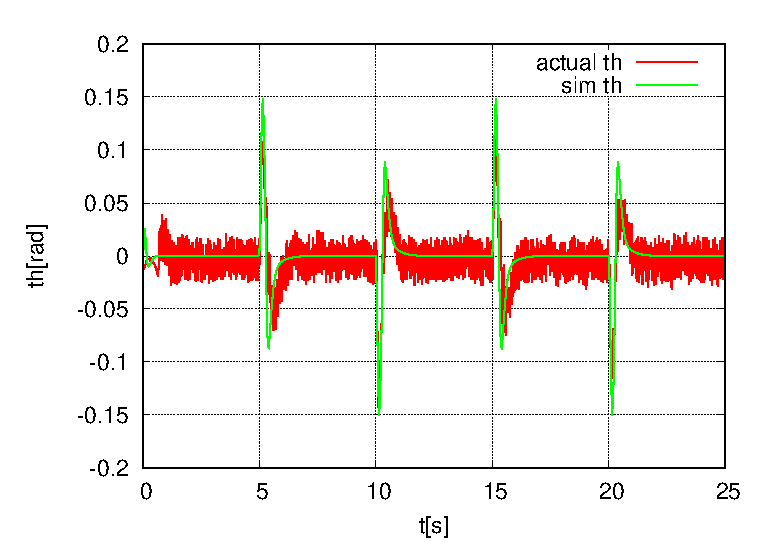
\includegraphics[width=1.0\linewidth]{case3_th.eps}
            \caption{図\ref{case03_th}: パターン03の振子角度}
            \label{case03_th}
        \end{center}
    \end{minipage}
\end{figure}

% --- patter 04 --- %
\begin{figure}[htbp]
    \begin{minipage}{0.5\hsize}
        \begin{center}
            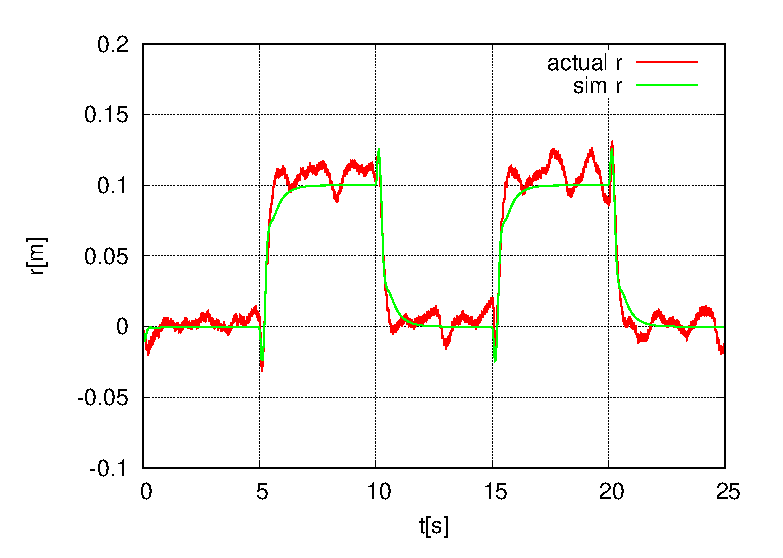
\includegraphics[width=1.0\linewidth]{case4_r.eps}
            \caption{図\ref{case04_r}: パターン04の台車位置}
            \label{case04_r}
        \end{center}
    \end{minipage}
    \begin{minipage}{0.5\hsize}
        \begin{center}
            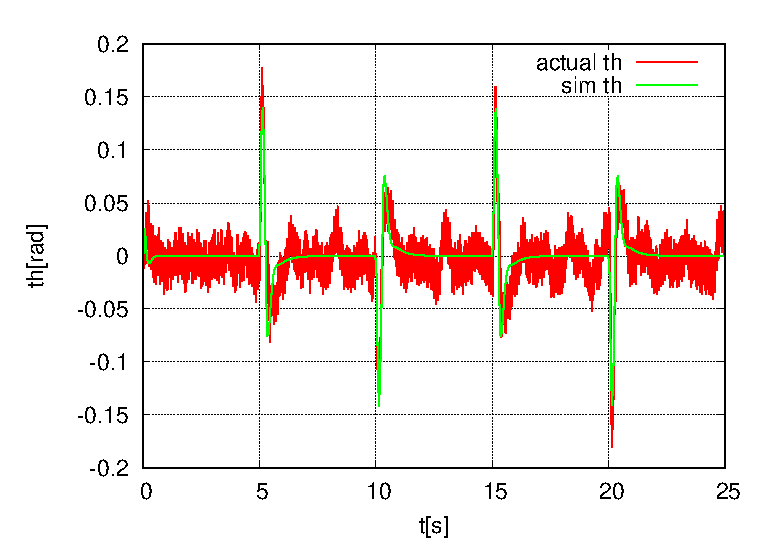
\includegraphics[width=1.0\linewidth]{case4_th.eps}
            \caption{図\ref{case04_th}: パターン04の振子角度}
            \label{case04_th}
        \end{center}
    \end{minipage}
\end{figure}

% --- patter 05 --- %
\begin{figure}[htbp]
    \begin{minipage}{0.5\hsize}
        \begin{center}
            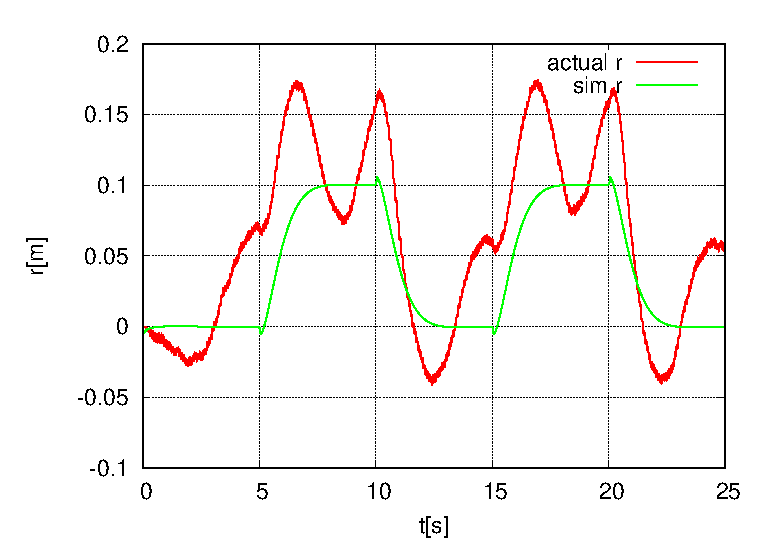
\includegraphics[width=1.0\linewidth]{case5_r.eps}
            \caption{図\ref{case05_r}: パターン05の台車位置}
            \label{case05_r}
        \end{center}
    \end{minipage}
    \begin{minipage}{0.5\hsize}
        \begin{center}
            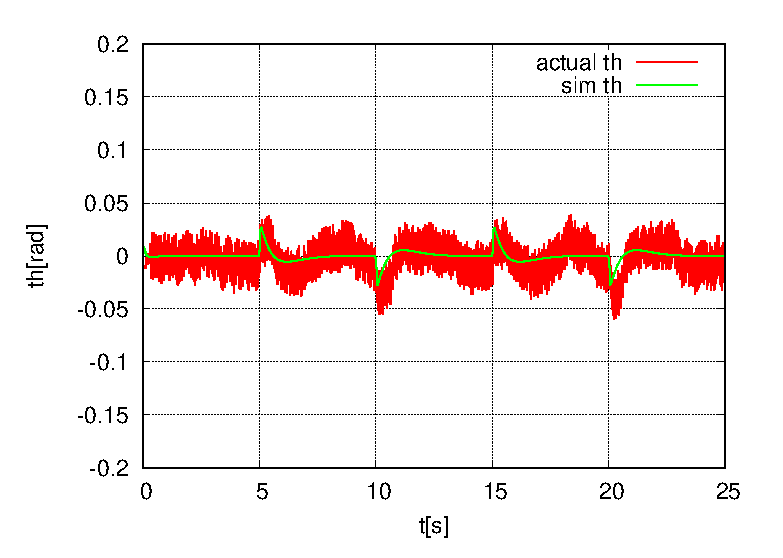
\includegraphics[width=1.0\linewidth]{case5_th.eps}
            \caption{図\ref{case05_th}: パターン05の振子角度}
            \label{case05_th}
        \end{center}
    \end{minipage}
\end{figure}

% --- patter 06 --- %
\begin{figure}[htbp]
    \begin{minipage}{0.5\hsize}
        \begin{center}
            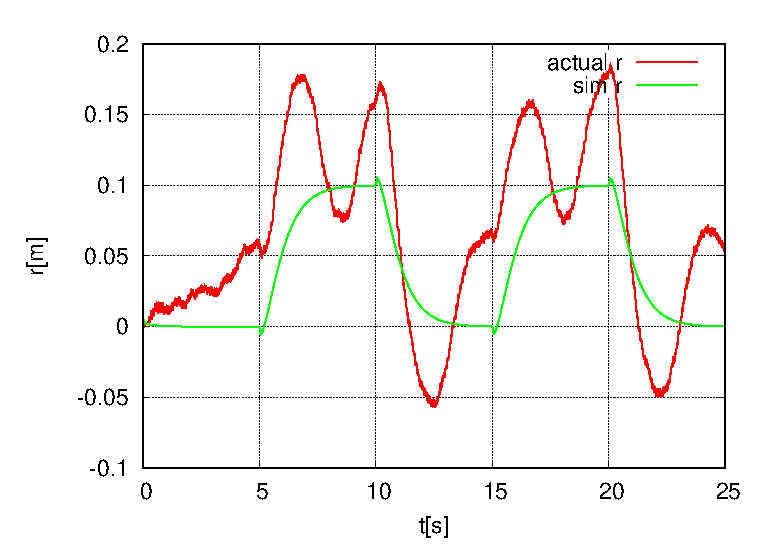
\includegraphics[width=1.0\linewidth]{case6_r.eps}
            \caption{図\ref{case06_r}: パターン06の台車位置}
            \label{case06_r}
        \end{center}
    \end{minipage}
    \begin{minipage}{0.5\hsize}
        \begin{center}
            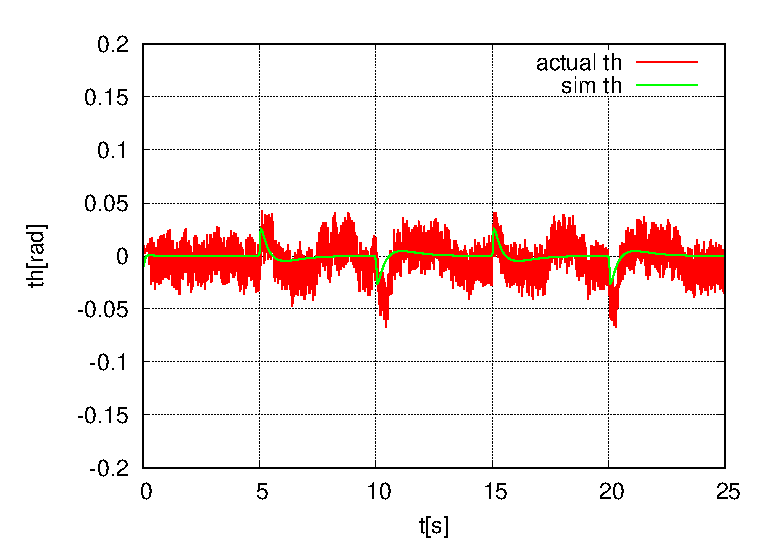
\includegraphics[width=1.0\linewidth]{case6_th.eps}
            \caption{図\ref{case06_th}: パターン06の振子角度}
            \label{case06_th}
        \end{center}
    \end{minipage}
\end{figure}

% --- patter 07 --- %
\begin{figure}[htbp]
    \begin{minipage}{0.5\hsize}
        \begin{center}
            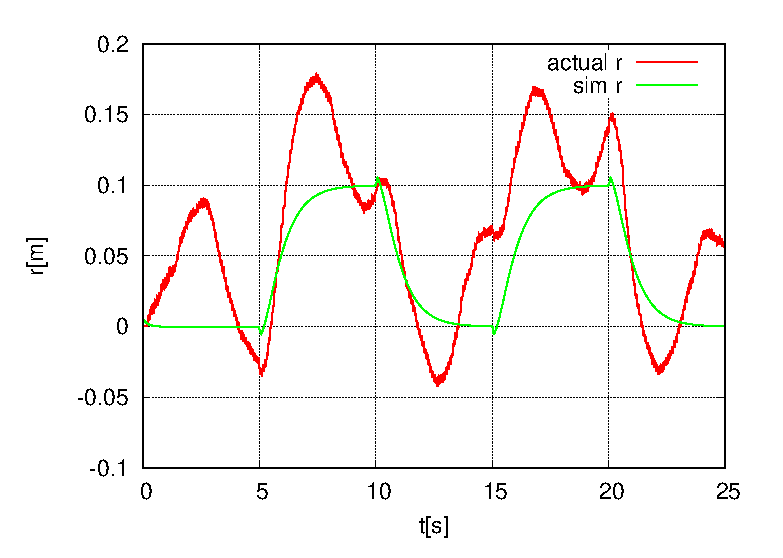
\includegraphics[width=1.0\linewidth]{case7_r.eps}
            \caption{図\ref{case07_r}: パターン07の台車位置}
            \label{case07_r}
        \end{center}
    \end{minipage}
    \begin{minipage}{0.5\hsize}
        \begin{center}
            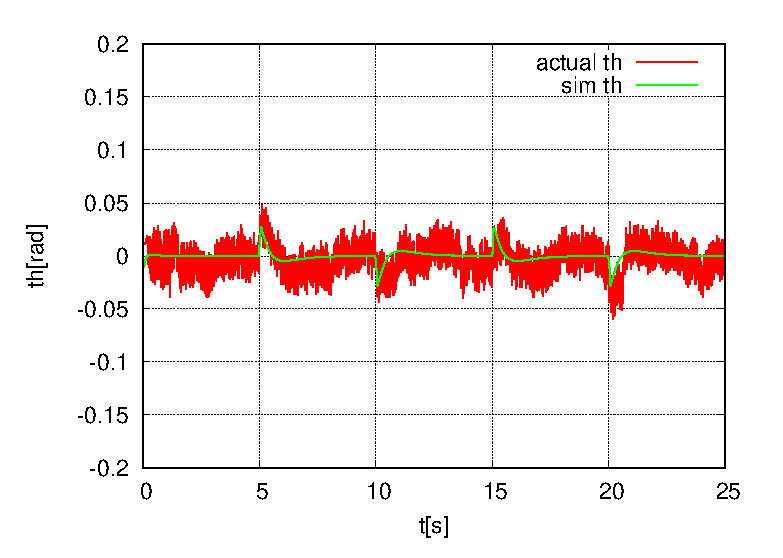
\includegraphics[width=1.0\linewidth]{case7_th.eps}
            \caption{図\ref{case07_th}: パターン07の振子角度}
            \label{case07_th}
        \end{center}
    \end{minipage}
\end{figure}

% --- patter 08 --- %
\begin{figure}[htbp]
    \begin{minipage}{0.5\hsize}
        \begin{center}
            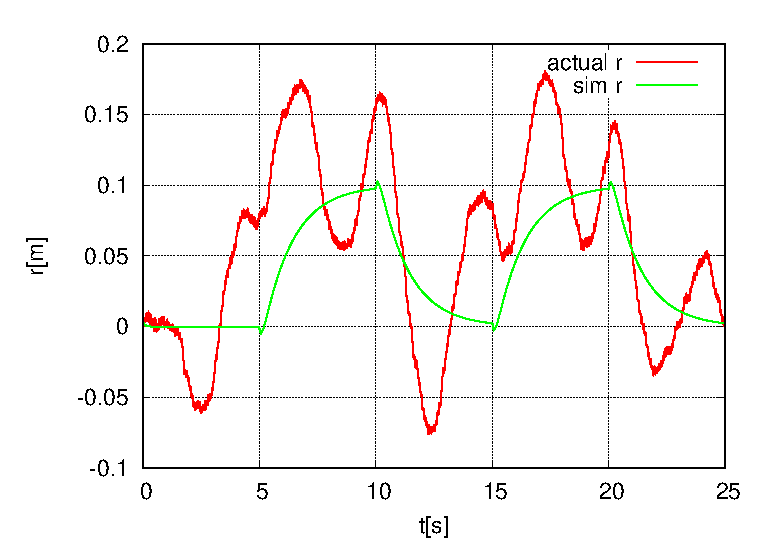
\includegraphics[width=1.0\linewidth]{case8_r.eps}
            \caption{図\ref{case08_r}: パターン08の台車位置}
            \label{case08_r}
        \end{center}
    \end{minipage}
    \begin{minipage}{0.5\hsize}
        \begin{center}
            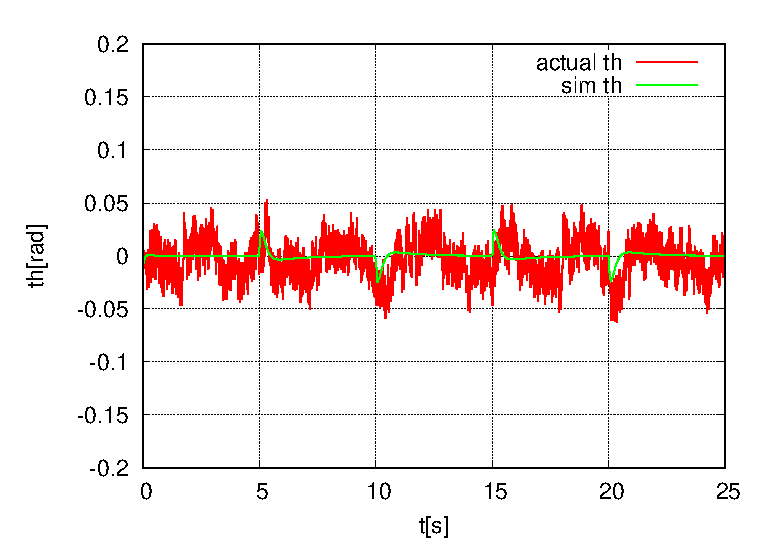
\includegraphics[width=1.0\linewidth]{case8_th.eps}
            \caption{図\ref{case08_th}: パターン08の振子角度}
            \label{case08_th}
        \end{center}
    \end{minipage}
\end{figure}

% --- patter 09 --- %
\begin{figure}[htbp]
    \begin{minipage}{0.5\hsize}
        \begin{center}
            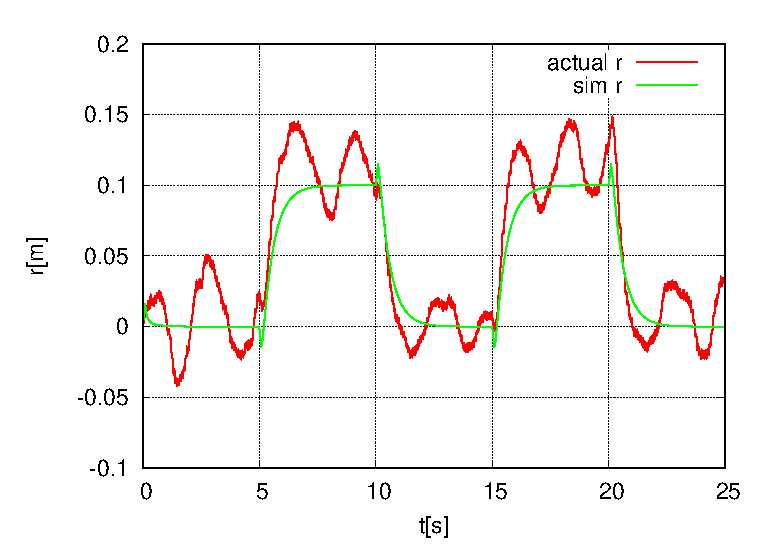
\includegraphics[width=1.0\linewidth]{case9_r.eps}
            \caption{図\ref{case09_r}: パターン09の台車位置}
            \label{case09_r}
        \end{center}
    \end{minipage}
    \begin{minipage}{0.5\hsize}
        \begin{center}
            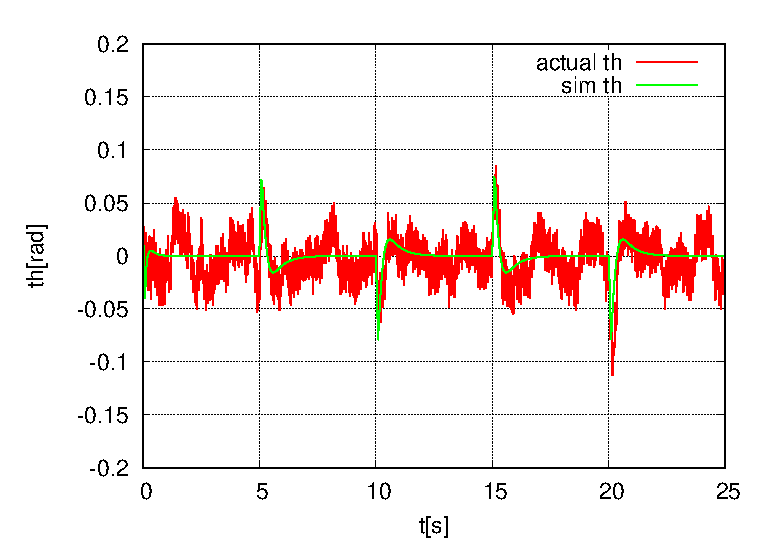
\includegraphics[width=1.0\linewidth]{case9_th.eps}
            \caption{図\ref{case09_th}: パターン09の振子角度}
            \label{case09_th}
        \end{center}
    \end{minipage}
\end{figure}

% --- patter 10 --- %
\begin{figure}[htbp]
    \begin{minipage}{0.5\hsize}
        \begin{center}
            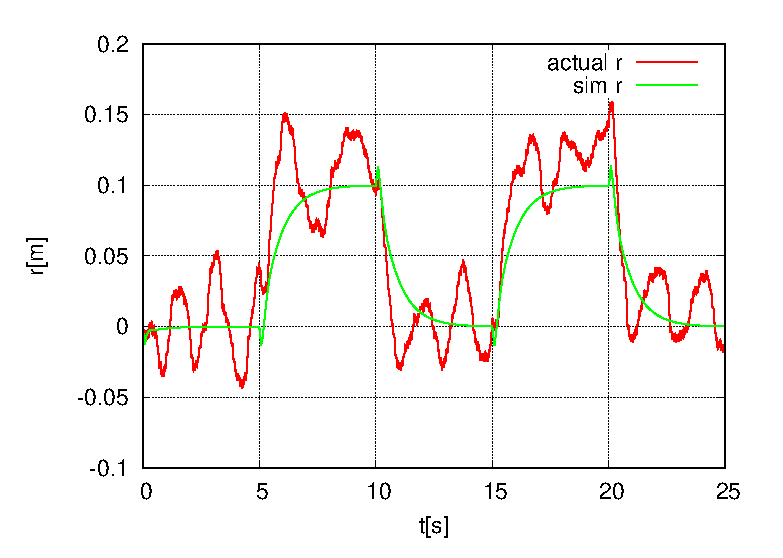
\includegraphics[width=1.0\linewidth]{case10_r.eps}
            \caption{図\ref{case10_r}: パターン10の台車位置}
            \label{case10_r}
        \end{center}
    \end{minipage}
    \begin{minipage}{0.5\hsize}
        \begin{center}
            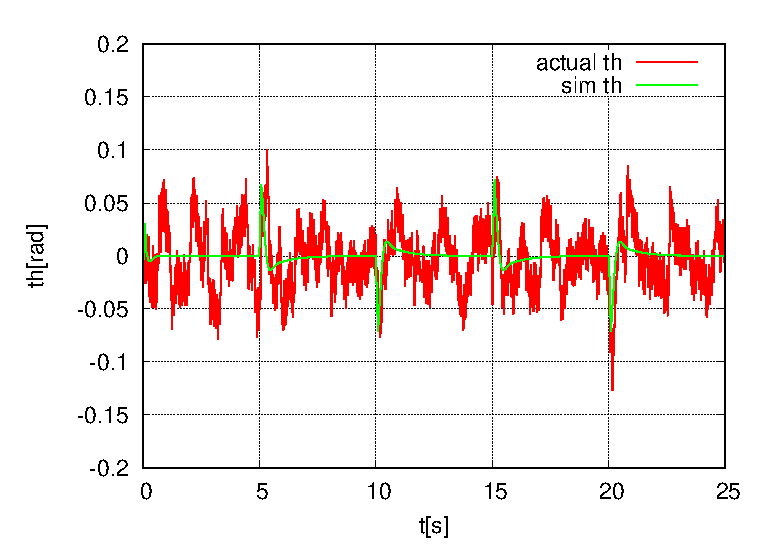
\includegraphics[width=1.0\linewidth]{case10_th.eps}
            \caption{図\ref{case10_th}: パターン10の振子角度}
            \label{case10_th}
        \end{center}
    \end{minipage}
\end{figure}

% --- patter 11 --- %
\begin{figure}[htbp]
    \begin{minipage}{0.5\hsize}
        \begin{center}
            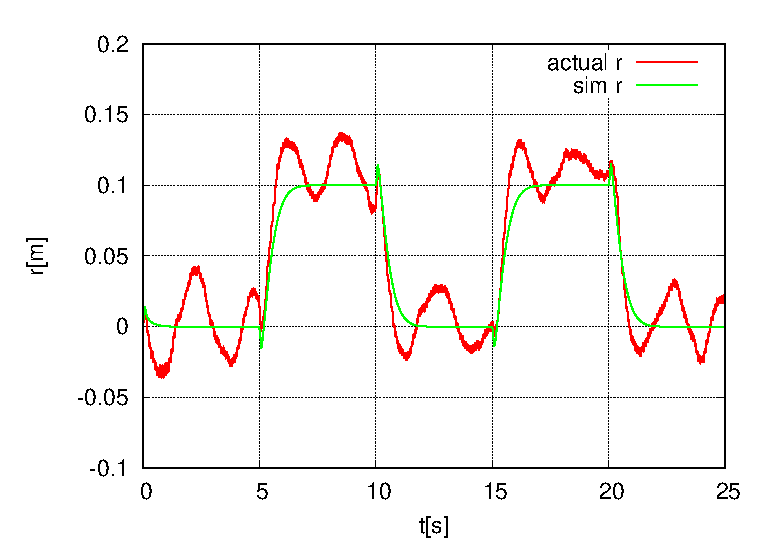
\includegraphics[width=1.0\linewidth]{case11_r.eps}
            \caption{図\ref{case11_r}: パターン11の台車位置}
            \label{case10_r}
        \end{center}
    \end{minipage}
    \begin{minipage}{0.5\hsize}
        \begin{center}
            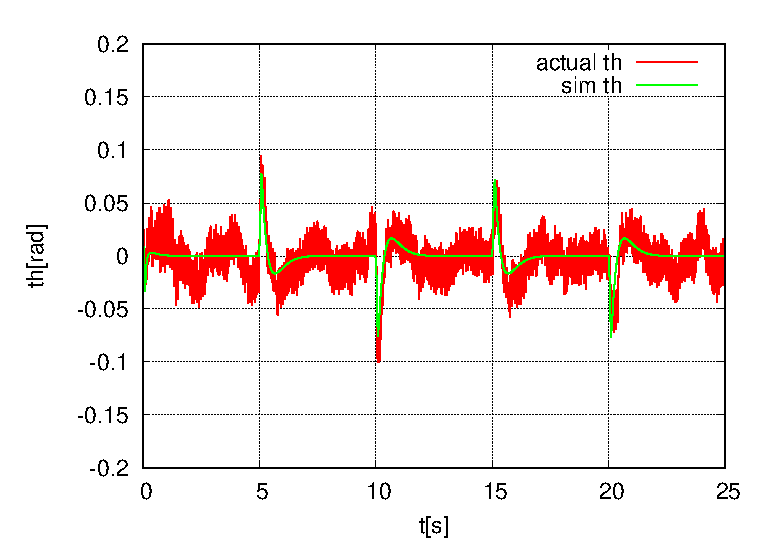
\includegraphics[width=1.0\linewidth]{case11_th.eps}
            \caption{図\ref{case11_th}: パターン11の振子角度}
            \label{case11_th}
        \end{center}
    \end{minipage}
\end{figure}

% --- patter 12 --- %
\begin{figure}[htbp]
    \begin{minipage}{0.5\hsize}
        \begin{center}
            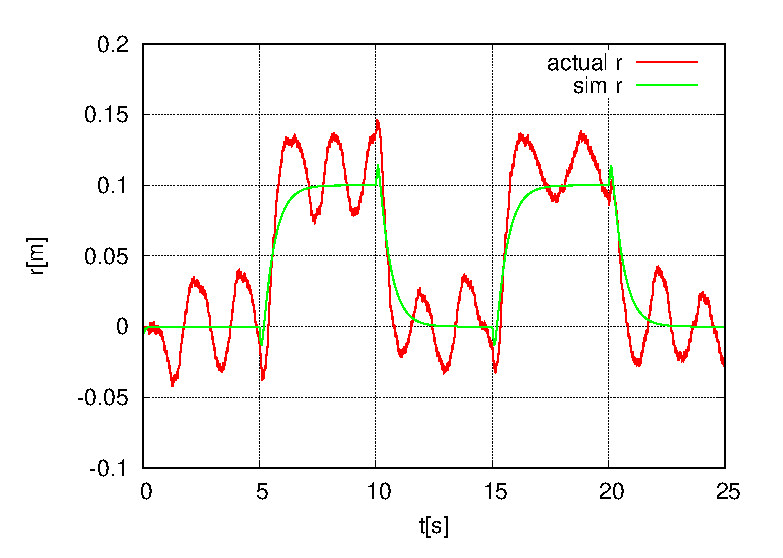
\includegraphics[width=1.0\linewidth]{case12_r.eps}
            \caption{図\ref{case12_r}: パターン12の台車位置}
            \label{case12_r}
        \end{center}
    \end{minipage}
    \begin{minipage}{0.5\hsize}
        \begin{center}
            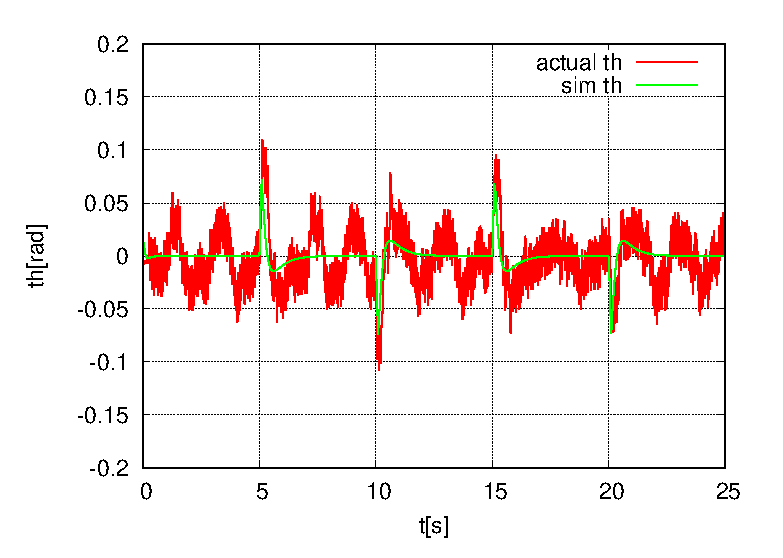
\includegraphics[width=1.0\linewidth]{case12_th.eps}
            \caption{図\ref{case12_th}: パターン12の振子角度}
            \label{case12_th}
        \end{center}
    \end{minipage}
\end{figure}

\subsection{目標値変更における安定化制御に関する考察}
\begin{itemize}
    \item 重み行列 \\
        振子角度よりも台車位置に重みを置いたパターン01からパターン03と、振子角度と台車位置に同等の
        重みを置いたパターン09からパターン12までを比較すると、台車位置に重みを置いた方が目標値への収束が
        早いことがわかる。逆に、振子角度に重みを置いたパターン03とパターン05では、パターン05の方が
        振子角度の振動が抑えられていることがわかる。
        よって、重み行列の各成分に対応した変位の応答を制御することができた。
    \item オブザーバ \\
        図\ref{case01_r}と図\ref{case02_r}を比較すると、オブザーバの極の実部が実軸負の方向に
        原点から離れているほうが、目標値への収束が早いと考えられる。しかし、今回行った実験の結果では、
        目標値への収束の速さに差異はなかった。今回は、$0.0 \to 0.5$[m]のような幅で安定化を行ったが、
        より目標値変更の幅を大きくすることでオブザーバの極による影響を観察できると考えられる。
        また、極の実部が負の方向に原点から離れている方が、ノイズを拾いやすくより振動的な応答を示している。
    \item サンプリング周期 \\
        サンプリング周期が小さいほど、より正確なシミュレーション、実験を行うことができる。
        すなわち、目標値への収束も早くなると言える。
        図\ref{case02_th}, 図\ref{case04_th}を比較すると、サンプリング周期が小さい図\ref{case04_th}
        の方が振動が抑えられ、目標値へ早く収束している。
\end{itemize}


\newpage
\subsection{振り上げ制御}
\subsection{振り上げ制御に関する考察}


% =============================== chapter 5 END =============================== %